\documentclass[10pt,letterpaper,onecolumn,draftclsnofoot]{IEEEtran}
\usepackage[margin=0.75in]{geometry}
\usepackage{graphicx}
\usepackage{listings}
\usepackage{color}
\usepackage{longtable}
\usepackage{tabu}
\definecolor{dkgreen}{rgb}{0,0.6,0}
\definecolor{gray}{rgb}{0.5,0.5,0.5}
\definecolor{mauve}{rgb}{0.58,0,0.82}

\lstset{frame=tb,
  language=Python,
  columns=flexible,
  numberstyle=\tiny\color{gray},
  keywordstyle=\color{blue},
  commentstyle=\color{dkgreen},
  stringstyle=\color{mauve},
  breaklines=true,
  breakatwhitespace=true,
  tabsize=4
}

\begin{document}
\begin{titlepage}
  \title{CS 434 - Spring 2016 - Final Project Report}
  \author{Garrett Smith, Cody Malick\\
  \texttt{smithgar@oregonstate.edu} | \texttt{malickc@oregonstate.edu}}
  \maketitle
  \vspace*{4cm}
  \begin{abstract}
      \noindent In this report, we examine four different algorithms for machine
      learning: linear regression, logistic regression, support vector machine,
      and decision tree. We apply these four algorithms to the same problem, spam
      classification, and examine how they perform, how they perform in different
      conditions, and how they compare to each other.

  \end{abstract}
\end{titlepage}

\tableofcontents
\clearpage
\section{Introduction}
Classification is a common problem in machine learning. There are many approaches,
some simple, some more complex, that all involve sorting a given set of items into
two or more classifications. The goal, of course, being able to quickly and efficiently
classify large sets of items into their correct classes. In our final project, we
have examined four seperate classification algorithms, and applied them all to the
same problem of classifying spam.

\section{The Data}
Our data set is a pre-processed set of spam from University of California Irvine,
the \texttt{Spambase Data Set}.\cite{spambase} The data set is comprised of the
following:
\begin{description}
  \item Number of Instances: 4601
  \item Number of Attributes: 57
  \begin{itemize}
    \item 48 continous real [0,100] attributes of type word\_freq\_WORD
    percentage of words in the e-mail that match WORD, i.e. 100 * (number of
    times the WORD appears in the e-mail) / total number of words in e-mail. A
    ``word'' in this case is any string of alphanumeric characters bounded by
    non-alphanumeric characters or end-of-string.

    \item 6 continuous real [0,100] attributes of type char\_freq\_CHAR]
    = percentage of characters in the e-mail that match CHAR, i.e. 100 *
    (number of CHAR occurences) / total characters in e-mail

    \item 1 continuous real [1,...] attribute of type capital\_run\_length\_average
    = average length of uninterrupted sequences of capital letters

    \item 1 continuous integer [1,...] attribute of type capital\_run\_length\_longest
    = length of longest uninterrupted sequence of capital letters

    \item 1 continuous integer [1,...] attribute of type capital\_run\_length\_total
    = sum of length of uninterrupted sequences of capital letters
    = total number of capital letters in the e-mail

    \item 1 nominal {0,1} class attribute of type spam
    = denotes whether the e-mail was considered spam (1) or not (0), i.e.
    unsolicited commercial e-mail.
  \end{itemize}
  \item Class Distribution
  \begin{itemize}
      \item Spam: 1813 (39.4\%)
      \item Non-Spam: 2788 (60.6\%)
  \end{itemize}
\end{description}

This data was great for a comparison set because we could look at the exact distribution
of data, what kind of data it was, what the different attributes meant, etc. Because we
did not have a separate training set, we built our training set out of about 750 entries
from the original training set of 4000. The training set contained both spam and non-spam
classified entries.

Now that we have the layout of the data, next we will examine our first algorithm,
linear regression.

\section{Linear Regression}
Linear regression is a very simple algorithm, designed to handle data in very simple
dimensions. We ran into a lot of problems trying to implement this algorithm over
a data set with over fifty features. After some trial and error, we decided that
applying this algorithm to a feature set this complex didn't make a lot of sense.
We were hitting a few percentage points in accuracy, and we believe that it was
purely luck that we got that many. Instead of thoroughly investigating linear regression,
we added support vector machine to our lineup of algorithms to examine. Before
jumping into a support vector machine, we will now examine the next closest thing
to linear regression, logistic regression.

\section{Logistic Regression}
Logistic regression is a form of classification that uses probability. We decided
to use logistic regression because it is a form of linear regression that is able
to handle large amounts of features with relative accuracy, and often yields good
results in a binary classification problem. 
	\subsection{Implementation}
	We implemented logistic regression by using the \texttt{scikit-learn} library
	in python. \texttt{scikit-learn} is a great library that has several implementations
	available and an extremely simple setup process. We used the \texttt{linear\_model.LogisticRegression}
	module.
	As far as execution, we first set it up with the appropriate features, and 
	got surprisingly good results right out of the box. With default settings 
	(no regularization, default penalty of l2), we achieved ~95\% accuracy on the
	 training set, and ~88\% accuracy on the test set. We experimented with different
	 regularization values from .1, high regularization, to 1.0, no regularization.
	 
	 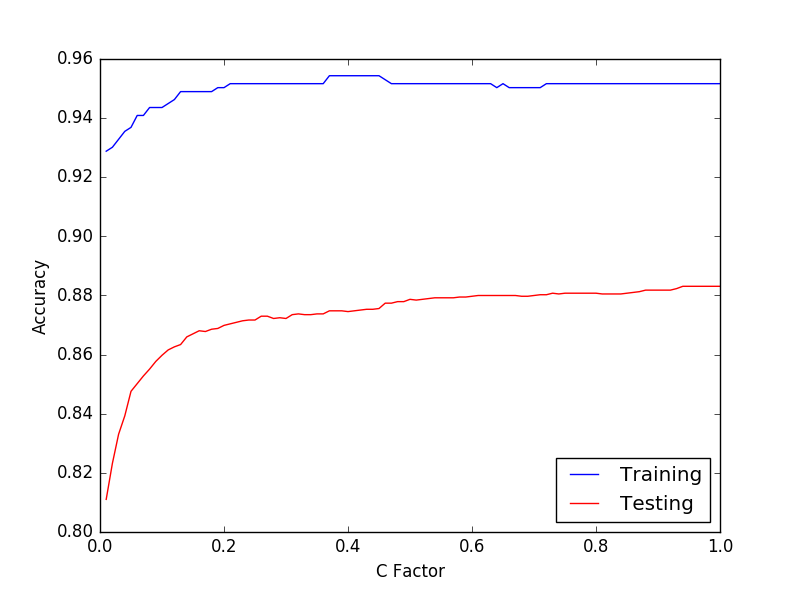
\includegraphics[scale=.75]{../logistic/l2_penalty}
	 
	 
	 Surprisingly, we only saw an increase in accuracy as regularization decreased. From
	 this behavior we can extrapolate that our data has few to no outliers skewing the
	 data in an unhelpful way. Next we tried applying l1 penalty instead of l2:
	 
	 
	 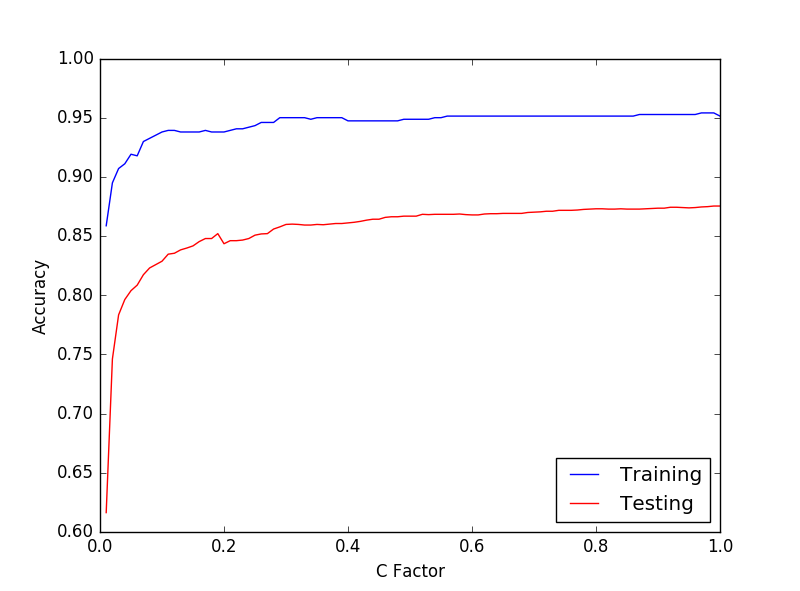
\includegraphics[scale=.75]{../logistic/l1_penalty}
	 
	 
	 With l1 penalty we see it takes quite a bit longer for the accuracy to peak, and 
	 overall there is a lower overall accuracy of about 3\%. This is expected as l1 
	 penalty is designed for data sets with sparse data, while l2 is better for larger,
	 more complete data sets.
	 
\section{Support Vector Machine}
\section{Decision Tree}

\section{Conclusion}

\clearpage
\section{Appendix A - Linux Structs}

\begin{lstlisting}

for future code samples

\end{lstlisting}

\section{Bibliography}
\bibliographystyle{IEEEtran}
\bibliography{final}

\end{document}
